\documentclass{article}
\usepackage{graphicx}
\topmargin=0.0in
\oddsidemargin=0.0in
\evensidemargin=0in 
\textwidth=6.5in
\marginparwidth=0.5in
\headheight=0pt 
\headsep=0pt
\textheight=9.0in
\newcommand\tab[1][3cm]{\hspace*{#1}}
 \begin{document}

 \begin{center}
 	 {
 	 	\large { SHUBHAM BARANWAL}
 	 }
 	
 \end{center}
 \hrule
 \begin{flushleft}
 	NIT Meghalaya, Bijni Complex, 		\hspace{1.7in}    		    Contact: 9436346271            \\
 	Laitumkhrah Shillong-793003  , 		\hspace{1.8in}		   e-mail id: shubhambaranwal2000@gmail.com\\
 	Meghalaya(India)     \\
\end{flushleft}

\vspace{-0.3in}

\begin{figure}[h]
	\hspace{4.4in}
	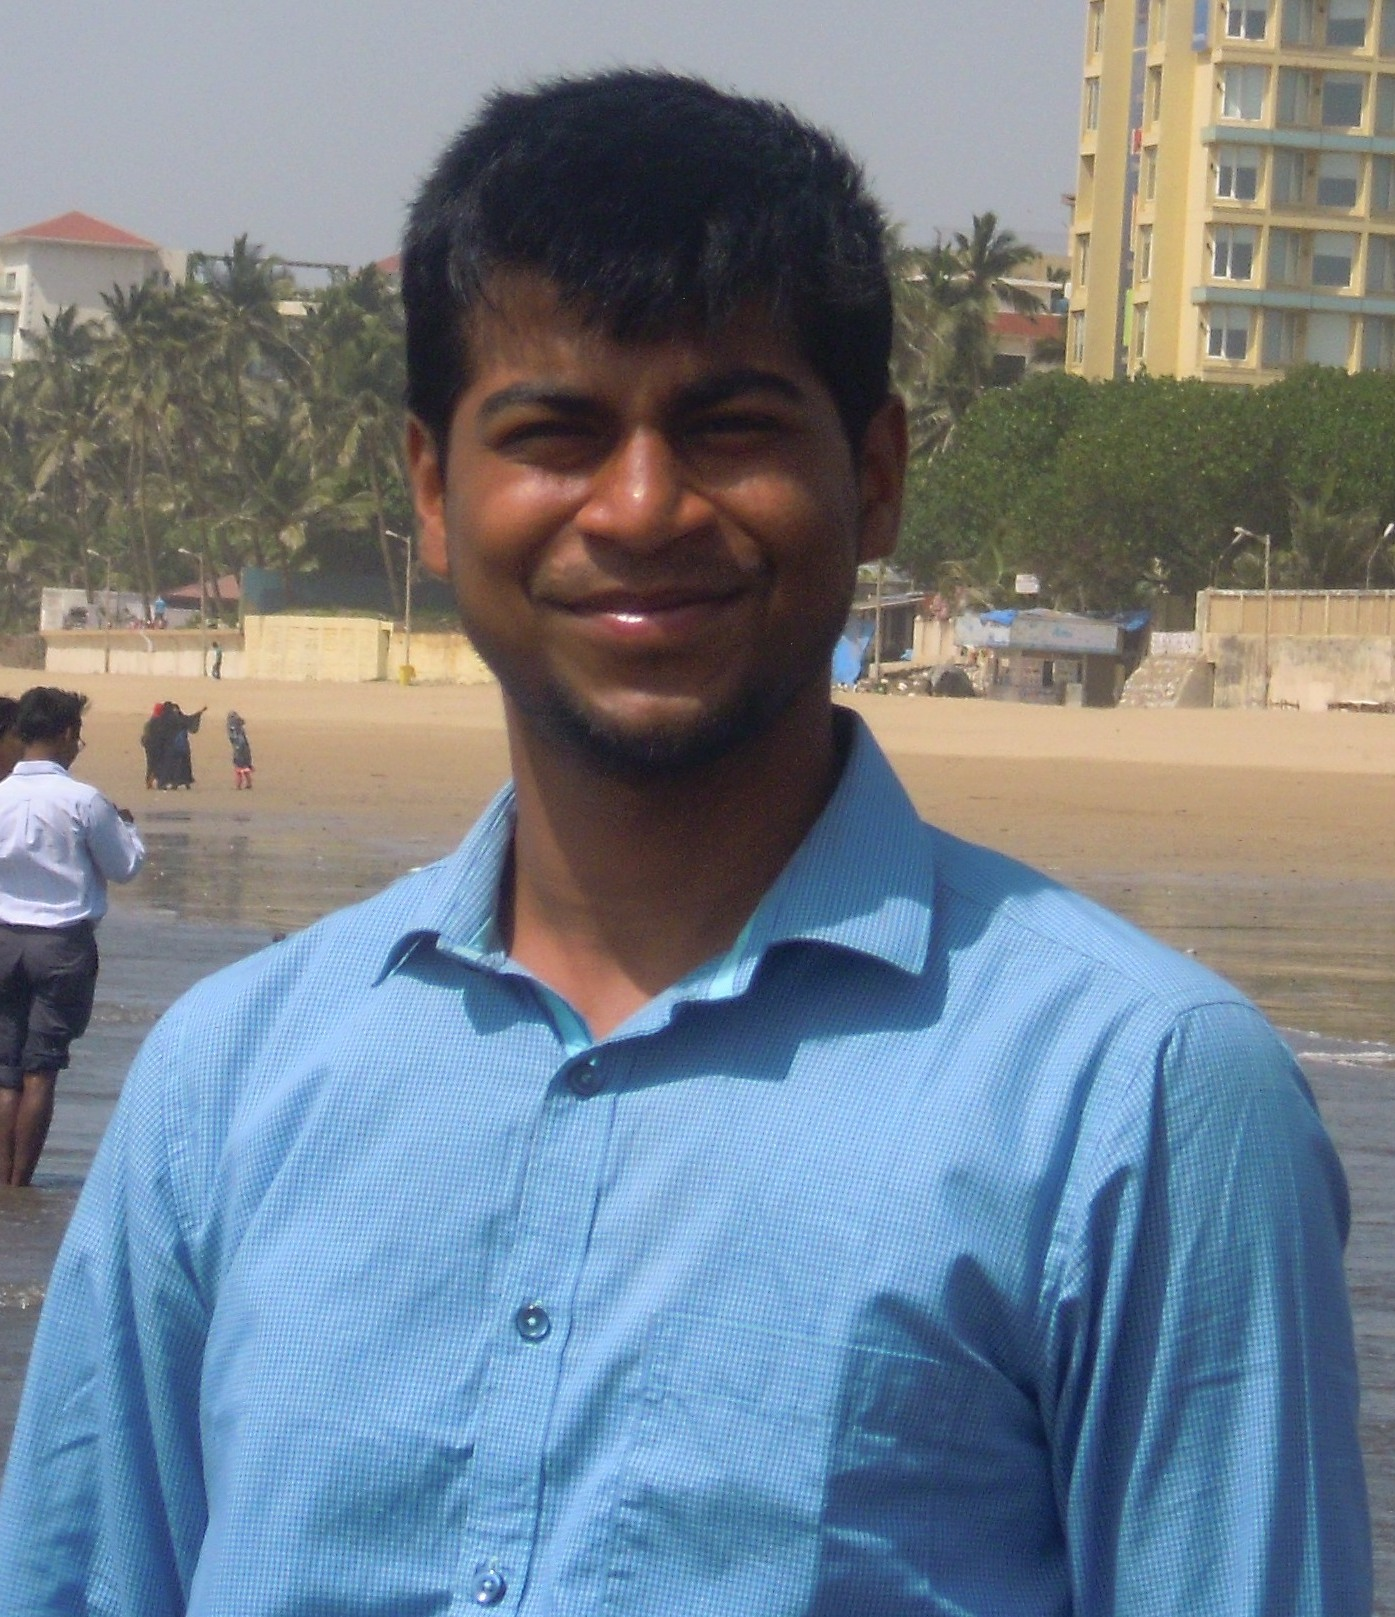
\includegraphics[width=90px]{shubham}
\end{figure}

%objective%

\begin{flushleft}
	\vspace{0.2in}
	\textbf{OBJECTIVE}
	
	\vspace{-0.20in}
	\hspace{1.4in}
	To enhance knowledge in the field of Embedded System and solve real-world \\
	\hspace{1.4in} problems
	
\end{flushleft}

 %  education %
 \begin{flushleft}
 	\vspace{0.3in}
 	\textbf{EDUCATION}
 	\hspace{0.1in}
 	\begin{tabular}{|c|c|c|c|c|}
 		\hline
 		Degree & School/College & Board/University & Passing Year & Percentage/CGPA   \\
 		\hline
 		B.tech & National Insitute & National Insitute & 2017 &8.34\\
 		E.E.E  & of Technology, Meghalaya & of Technology, Meghalaya & & (till 5th sem) \\
 		(pursuing) & & & &\\
 		\hline
 		AISSCE & Army Public School, & Central Board of & 2013 &90.83\\
 		(Class 12)  & Shillong & of Secondary Education & &\\
 		\hline
 		AISSE & Army Public School, & Central Board of & 2011 &10\\
 		(Class 10)  & Shillong & of Secondary Education & &\\
 		\hline
 		
 	\end{tabular}
 \end{flushleft}

% project %
\begin{flushleft} 
	\vspace{0.3in}
	\textbf{PROJECTS}
	\begin{enumerate}
		\vspace{-0.29in}
		\addtolength{\itemindent}{1.359in}
		\item  Autonomous Robot on Hazardous Waste Disposal Theme in e-YANTRA'15
		\item  Line Follower Robot using ATMEGA 16 Microcontroller
		\item Working on Smart Home Theme of Robotics and IOT Club, NIT
		Meghlaya
	\end{enumerate}
\end{flushleft}

  %research and publication %
  \begin{flushleft} 
  	\vspace{0.3in}
  	\textbf{RESEARCH \& \\ PUBLICATION}
  	\begin{itemize}
  		\vspace{-0.44in}
  		\addtolength{\itemindent}{1.359in}
  		\item  PV and QV curve analysis on IEEE-30 bus system
  	\end{itemize}
  \end{flushleft}


%training and internship %
\begin{flushleft} 
	\vspace{0.3in}
	\textbf{TRAINING \& \\ INTERNSHIP}
	\begin{enumerate}
		\vspace{-0.44in}
		\addtolength{\itemindent}{1.359in}
		\item  HINDALCO in Summer 2015
		\item  E- Yantra Summer Internship 2016 (in near future)
	\end{enumerate}
\end{flushleft}

 
 %technical skill %	
 \begin{flushleft}
 	\vspace{0.4in}
 	\textbf{TECHNICAL  \\ SKILL}
 	\begin{itemize}
 		\vspace{-0.45in}
 		\addtolength{\itemindent}{1.359in}
 		\item  Familiar in following Programming Languages
 		{\begin{itemize}
 				\addtolength{\itemindent}{1.359in}
 				\item C
 				\item C++
 				\item Embedded C
 				\item Assembly Language
 				
 			\end{itemize}
 		}  
 		\item Worked on following  Micro Controller and Micro-Processor
 		{\begin{itemize}
 				\addtolength{\itemindent}{1.359in}
 				\item 8081 Microcontroller
 				\item ATMEGA 2560 Microcontroller
 				\item ATMEGA 16 Microcontroller
 				\item 8085 and 8086 Microprocessor
 				
 			\end{itemize}
 		} 
 		\item  Familiar with following Simulation Software
 		{\begin{itemize}
 				\addtolength{\itemindent}{1.359in}
 				\item Proteus 8
 				\item Keil uVision
 				\item MATLAB  	
 				\item ATMEL Studio
 				\item Power System Simulator for Engineers (PSS@E)		
 			\end{itemize}
 		} 
 		
 	\end{itemize}
 \end{flushleft}
 
   	%soft skill%
   	\begin{flushleft} 
   		
   		\vspace{0.3in}
   		\textbf{SOFT SKILL}
   		\begin{enumerate}
   			\vspace{-0.30in}
   			\addtolength{\itemindent}{1.559in}
   			\item Leadership 
   			\item Teamwork
   			\item Management 
   			\item Communication
   		\end{enumerate}
   	\end{flushleft}
 
 
 
 %extra curricular activities%
 \begin{flushleft} 
 	\vspace{0.3in}
 	\textbf{EXTRA - \\CURRICULAR \\ACTIVITIES }
 	\begin{itemize}
 		\vspace{-0.65in}
 		\addtolength{\itemindent}{1.359in}
 		\item  Worked as Co-Coordinator and Coodinator in organising Techincal and \\
 		\hspace{1.3in}
 		Cultural festival of NIT Meghalaya\\ 
 		\item Volunteered in Social works through NSS
 		\item Volunteered in NIT Awareness Drive programme conducted by NIT Meghalaya
 		\item Volunteered in organising Shillong Run
 	\end{itemize}
 \end{flushleft}
 
  \begin{flushleft} 
  	\vspace{0.4in}
  	\textbf{CO- \\CURRICULAR \\ACTIVITIES }
  	\begin{enumerate}
  		\vspace{-0.65in}
  		\addtolength{\itemindent}{1.359in}
  		\item  Winner of e-Yantra-2015 under theme Hazardous Waste Disposal. 
  		\item  Winner of Stair Climber event organized by TechXtra-15(annual Technical\\\hspace{3.4cm} festival),Tezpur University.
  		\item  Runner up of Track Minion event organized by TechXtra-15 (annual \\\hspace{3.4cm}Technical festival), Tezpur University.  
  		\item  Winner of Line follower Robot event organized by Cognitia-13(annual \\\hspace{3.4cm}Technical festival), NIT Meghalaya.
  		
  	\end{enumerate}
  \end{flushleft}
 
 
 %personal details 	%
 
 \begin{flushleft}
 	\vspace{0.4in}
 	\textbf{PERSONAL \\ DETAILS} 
 	\hspace{0.8in}Father's name: \hspace{0.13in} Sanjay Kumar \\
 	\hspace{1.55in}Mother's name: \hspace{0.08in} Mridula Baranwal\\
 	\hspace{1.55in}Sex:\hspace{0.85in} Male\\
 	\hspace{1.55in}Date of birth:\hspace{0.255in} 27th March 1996	\\
 	\hspace{1.55in}Nationality:\hspace{0.45in}Indian\\
 	\hspace{1.55in}Marital status:\hspace{0.28in}Unmarried
 	
 \end{flushleft}
 
 %reference%
 \begin{flushleft}
 	\vspace{0.2in}
 	\textbf{REFERENCE} \hspace{0.30in} : Google
 \end{flushleft}
 
 %declaration%
 \begin{flushleft}
 	\vspace{0.2in}
 	\textbf{DECLARATION} \hspace{0.30in} : I hereby declare that all the details furnished above are true to the best of\\ 
 	\hspace{1.6in} my knowledge and belief.
 \end{flushleft}
 
 
 %	date%
 \begin{flushleft}
 	\vspace{0.2in}
 	\textbf{DATE} \hspace{1.05in} : 25th May 2016
 \end{flushleft}
\end{document}